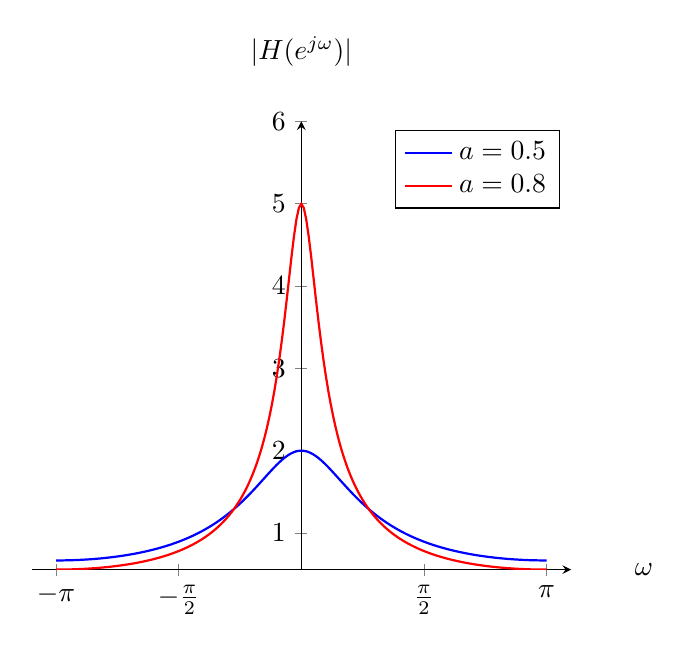
\begin{tikzpicture}
	
	\begin{axis}[
		xlabel=$\omega$,
		ylabel=$|H(e^{j\omega})|$,
		axis lines = middle,
		xmin = -1.1*pi,
		xmax = 1.1*pi,
		ymax = 6,
    	xtick={-3.14159, -1.5708, 1.5708, 3.14159},
    	xticklabels={$-\pi$, $-\frac{\pi}{2}$, $\frac{\pi}{2}$, $\pi$},
    	y label style={at={(axis description cs:0.5,1.1)},anchor=south},
    	x label style={at={(axis description cs:1.1,0)},anchor=west},    	
	]
	\def\a{0.5}
	\addplot[blue, thick, domain=-pi:pi, samples=201] {1/sqrt(1 + \a^2 - 2*\a*cos(deg(x)))};
	\def\a{0.8}
	\addplot[red, thick, domain=-pi:pi, samples=201] {1/sqrt(1 + \a^2 - 2*\a*cos(deg(x)))};
	\legend{$a=0.5$, $a=0.8$}
	\end{axis}
\end{tikzpicture}